\documentclass{article}

% Language setting
% Replace `english' with e.g. `spanish' to change the document language
\usepackage[english]{babel}

% Set page size and margins
% Replace `letterpaper' with `a4paper' for UK/EU standard size
\usepackage[letterpaper,top=2cm,bottom=2cm,left=3cm,right=3cm,marginparwidth=1.75cm]{geometry}

% Useful packages
\usepackage{amsmath}
\usepackage{graphicx}
\usepackage[colorlinks=true, allcolors=blue]{hyperref}
\usepackage{subfigure}

\newcommand{\todo}[1]{{\sf[{\footnotesize{{\color{blue} To Do: #1}}]}}}

\title{TDT4265 Computer Vision and Deep Learning - Final Project}
\author{Project group 102: Marco Kugler, Pia Bauspieß}

\begin{document}
\maketitle

\section*{Task 1: Dataset exploration}

The original dataset consists of 1,905 LIDAR-images (1604 for traning, 301 for validation) collected in traffic in the area around NTNU campus Gløshaugen in Trondheim, Norway. The updated version with additional images annotated by our fellow classmates and ourselves consists of a total of 16,6997 images (16,696 for training, 301 for validation). Each image is comprised of three 360° LIDAR-channels with a resolution of 128 pixels in height and 1,024 pixels in width. Within the dataset, moving objects in traffic out of the following eight object categories are annotated: car, truck, bus, motorcycle, bicycle, scooter, person, and rider. All other objects are are attributed to the background class.

For a first overview of the dataset, we visualised all images in randomly selected batches of 80 images for both the training data set, the updated traning dataset, and the validation set. In the first step, the three LIDAR channels are interpreted as RGB images as proposed in the task description. Subsequently, we investigated each image channel individually, as well as images that contain at least one object of a chosen category. An overview of this initial exploration for the original training dataset is given in Figure \ref{fig:overview}\footnote{Figure \ref{fig:overview} is merely supposed to show the methodology of our exploration, not the content of single images, which are therefore printed only at a small scale in this document.}, while the entire visualisation of the original training set, the updated training set, and the validation set can be accessed at \todo{enter link}.

\begin{figure}[h!]
    \centering
    \subfigure[]{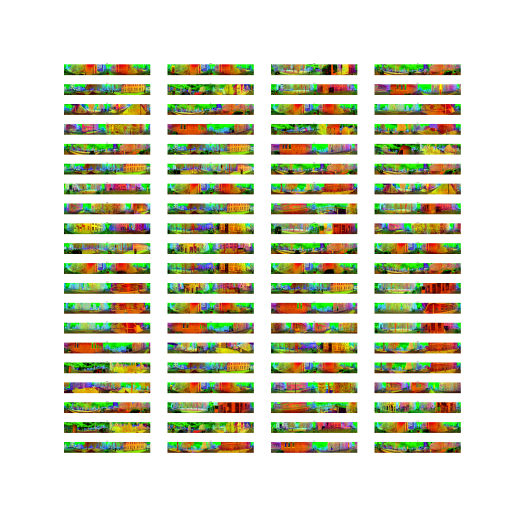
\includegraphics[width=0.16\textwidth]{image_overview/random_all_channels_train_small.png}} 
    \subfigure[]{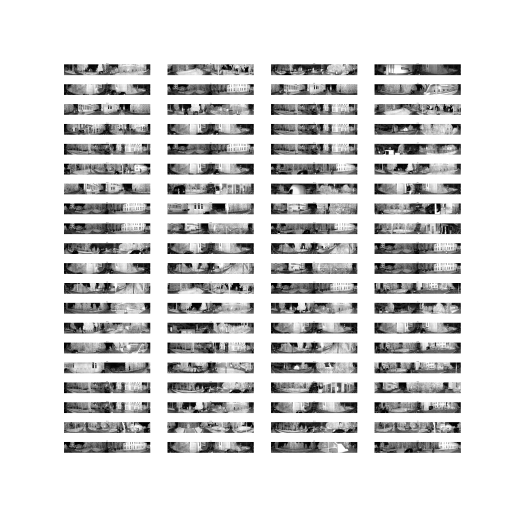
\includegraphics[width=0.16\textwidth]{image_overview/random_channel1_train_small.png}} 
    \subfigure[]{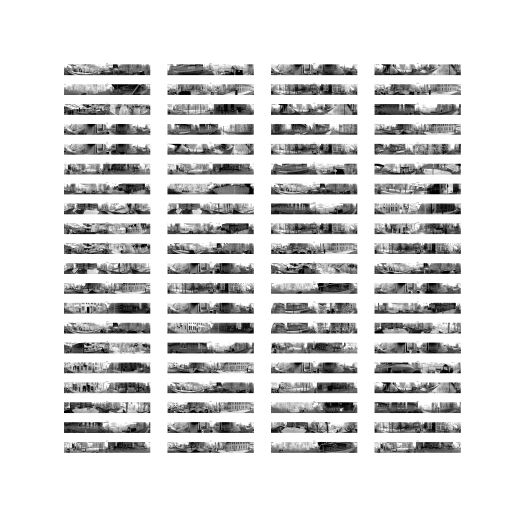
\includegraphics[width=0.16\textwidth]{image_overview/random_channel2_train_small.png}}
    \subfigure[]{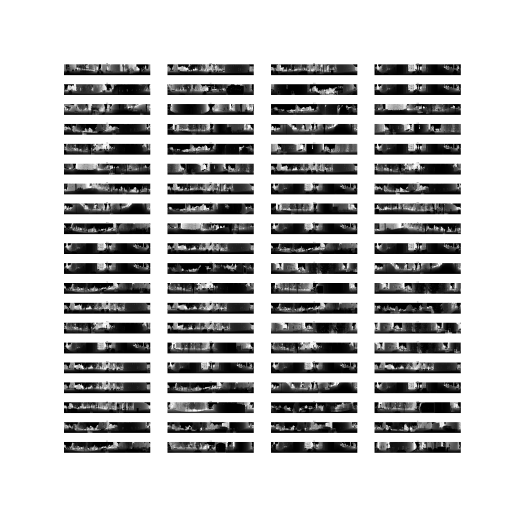
\includegraphics[width=0.16\textwidth]{image_overview/random_channel3_train_small.png}}
    \subfigure[]{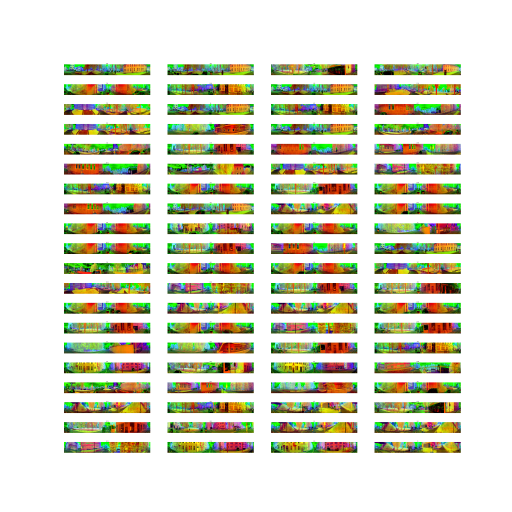
\includegraphics[width=0.16\textwidth]{image_overview/random_car(1)_train_small.png}}
    \subfigure[]{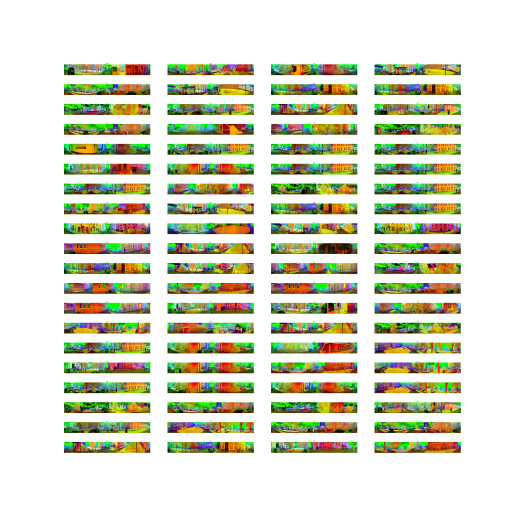
\includegraphics[width=0.16\textwidth]{image_overview/random_person(7)_train_small.png}}
    \caption{Randomly selected images from the original training set showing (a) all three channels combined (b) the first channel (depth) (c) the second channel (ambience) (d) the third channel (intensity) (e) cars (f) persons.}
    \label{fig:overview}
\end{figure}

\subsection*{Quantitative analysis}
The prevalent object class in the original training set are cars (52.3\%), followed by persons (26.8\%) and riders of vehicles (8.7\%). This can be seen both from Figure \ref{fig:ratio}, which shows the ratio of labels over the original training set, the updated training set, and the validation set, as well as Figure \ref{fig:occurrence} (a), showing the total occurrence of labels in the training set, the updated training set, and the validation set. While this observation is roughly consistent with the updated extended training set (51.9\% cars, 32.3\% persons, 4.9\% bicycles), the distribution differs significantly from the validation set. Here, the most prevalent object class are persons (66.7\%), followed by cars (25.9\%) and riders (5.7\%). Notably, the validation set does not contain any images with trucks, bicycles, scooters or motorcycles. The existence of riders in the absence of any vehicles that transport riders (bicycles, scooters and motorcycles) in the validation set raises questions, which will be discussed in the following.

Figure \ref{fig:occurrence} offers more insight into correlations of annotated objects in single images in plots (b), (c), and (d).

\begin{figure}[t]
    \centering
    \subfigure[]{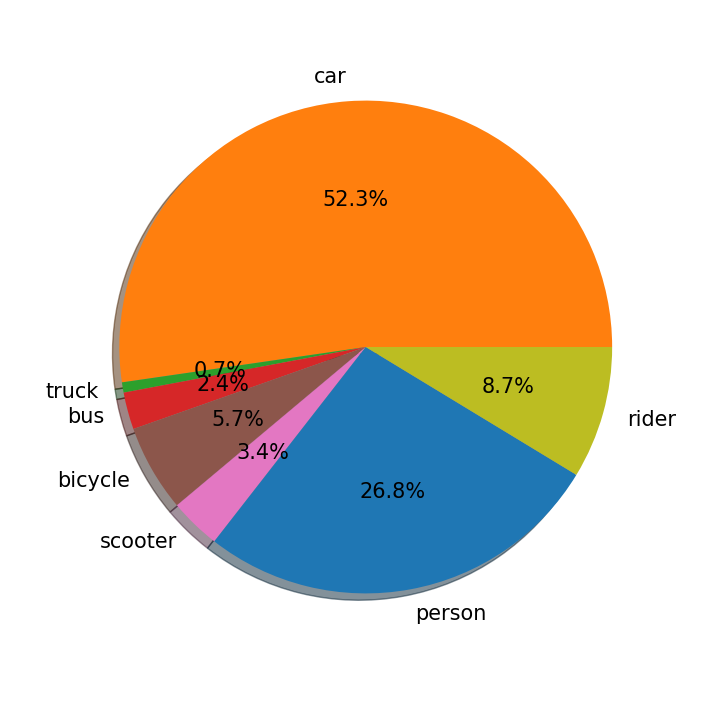
\includegraphics[width=0.32\textwidth]{label_distribution/train/label_ratio_train_cropped.png}}
    \subfigure[]{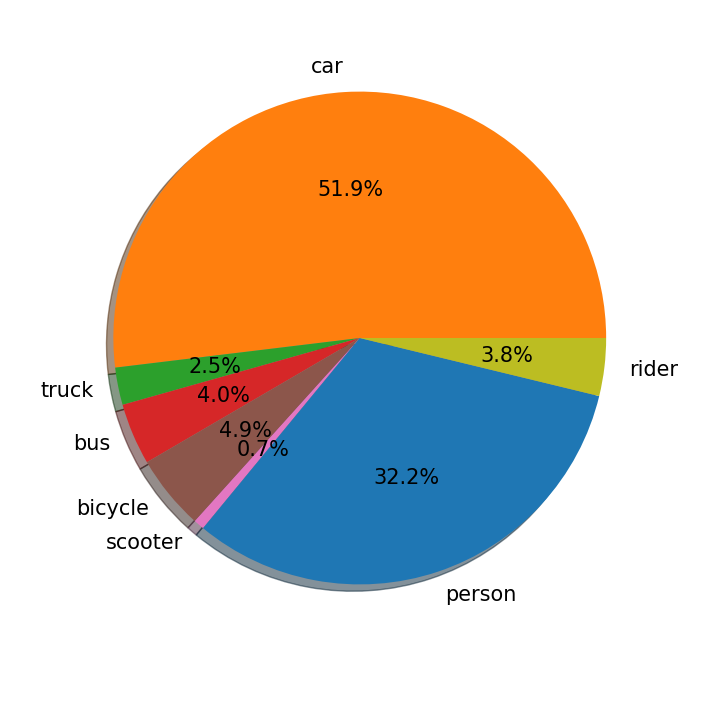
\includegraphics[width=0.32\textwidth]{label_distribution/extended_train/label_ratio_extended_train.png}} 
    \subfigure[]{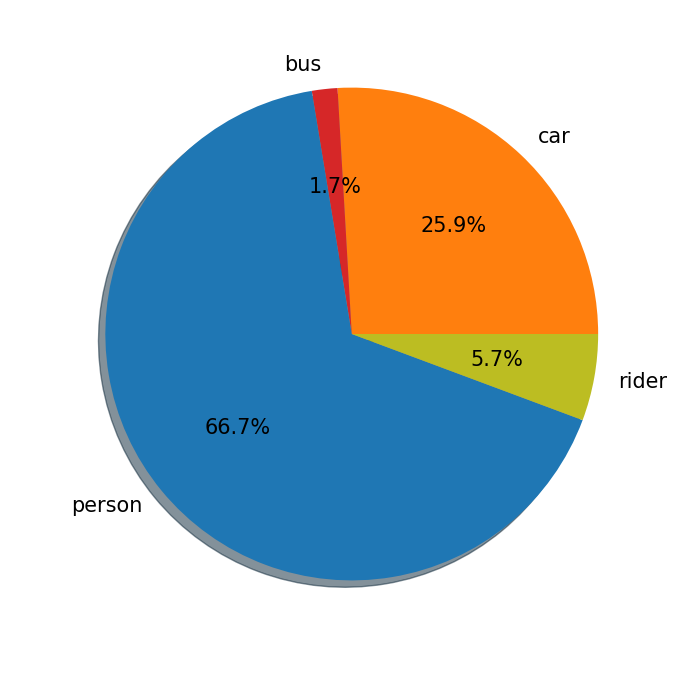
\includegraphics[width=0.32\textwidth]{label_distribution/val/label_ratio_val_cropped.png}} 
    \caption{Label ratios over (a) original training set (b) updated training set (c) validation set.}
    \label{fig:ratio}
\end{figure}

\begin{figure}[t!]
    \centering
    %\subfigure[]{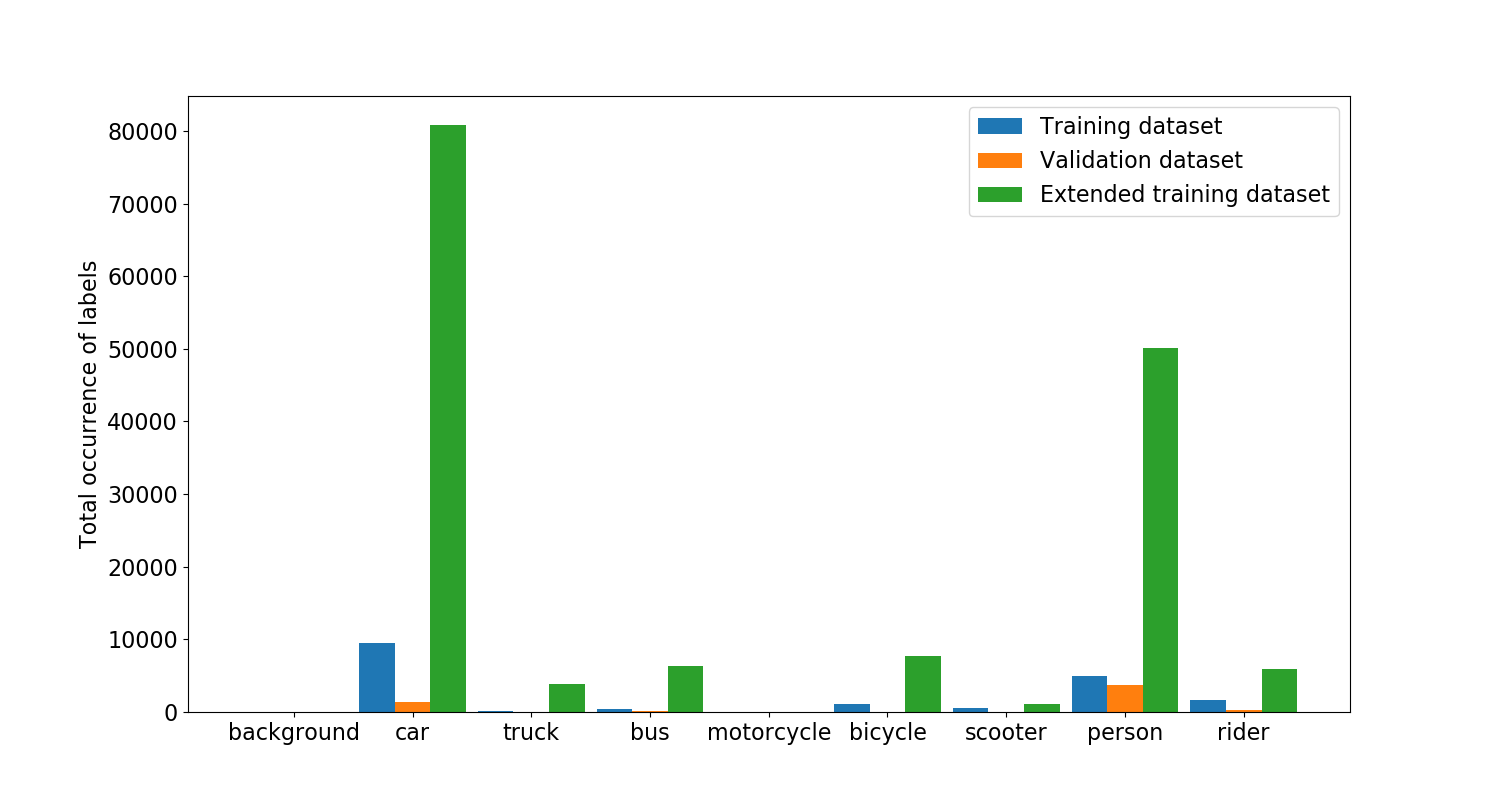
\includegraphics[width=0.49\textwidth]{label_distribution/comparison/total_occurence_comparison.png}}
    %\subfigure[]{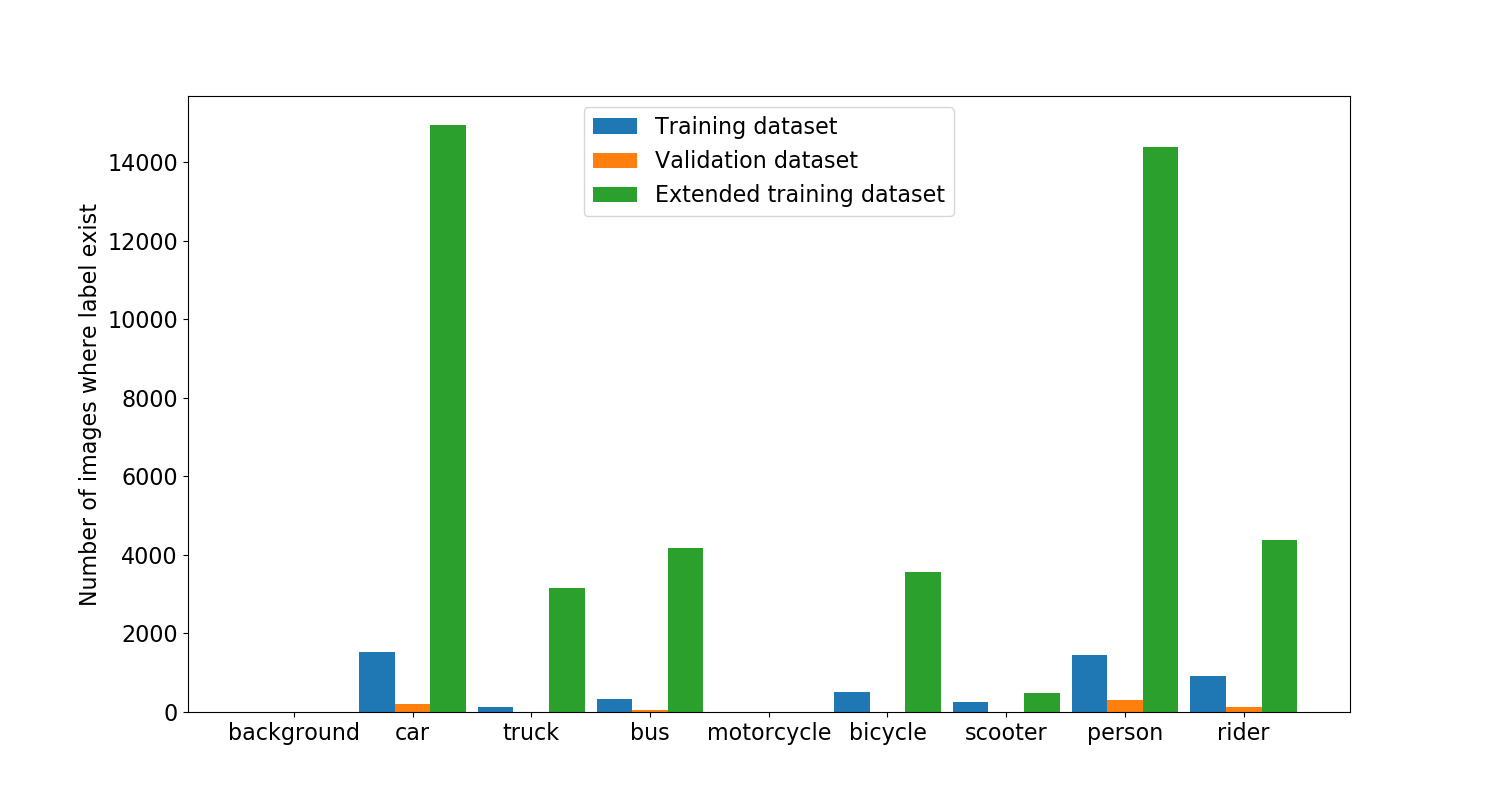
\includegraphics[width=0.49\textwidth]{label_distribution/comparison/number_images_where_label_exist_comparison.png}} 
    \subfigure[]{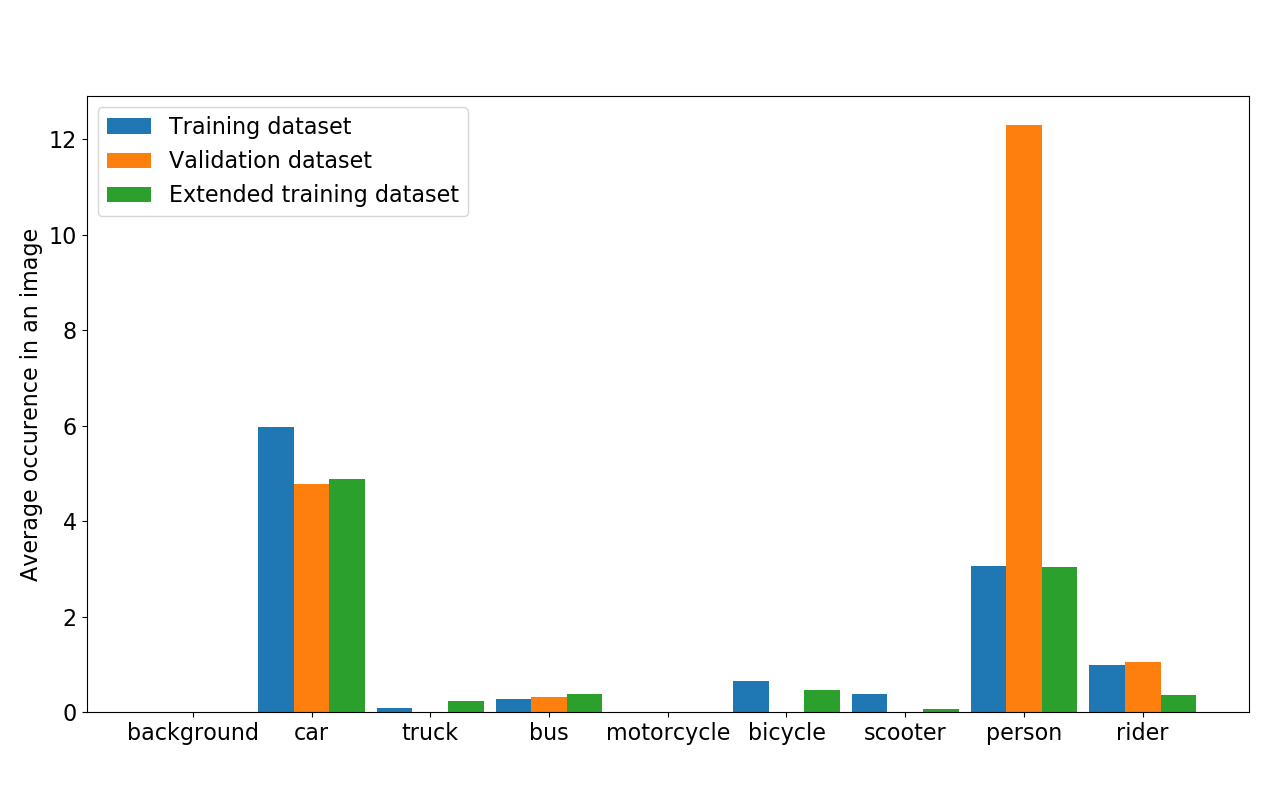
\includegraphics[width=0.49\textwidth]{label_distribution/comparison/avg_occ_comparison.png}} 
    \subfigure[]{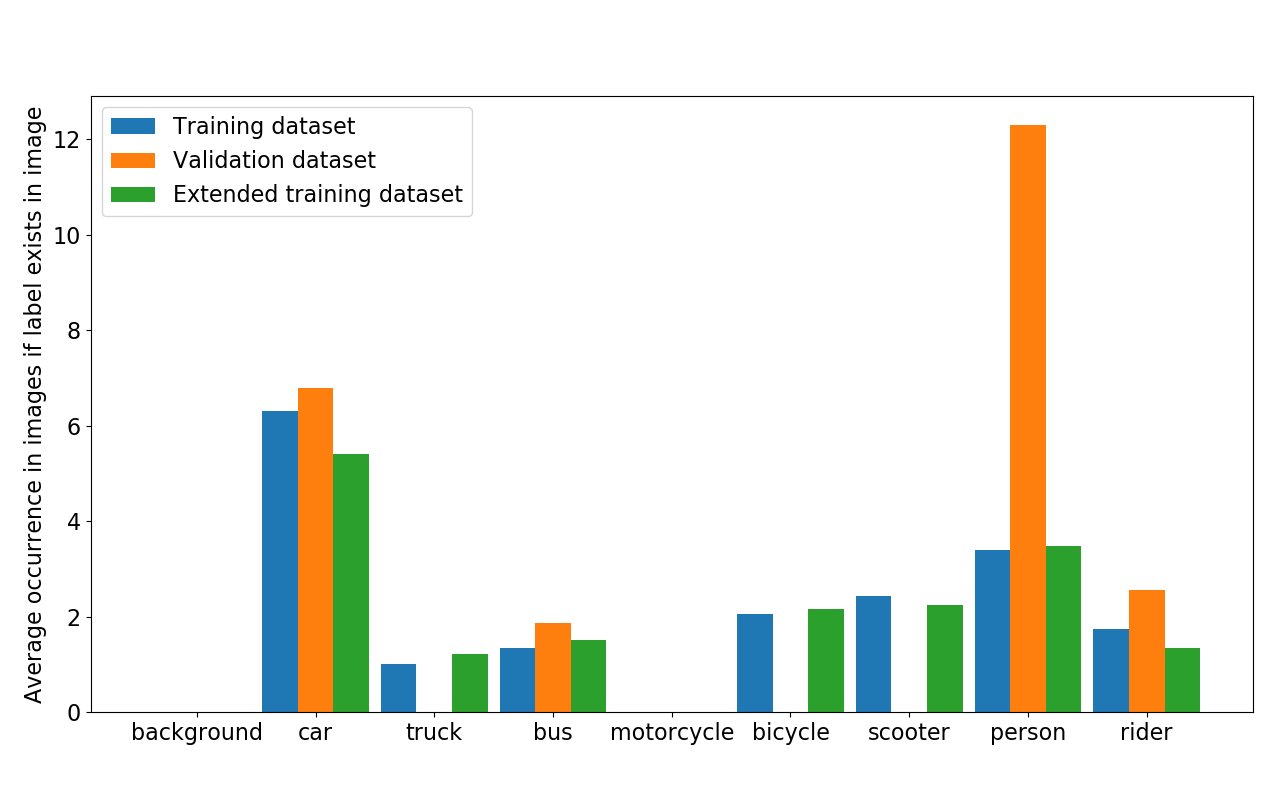
\includegraphics[width=0.49\textwidth]{label_distribution/comparison/avg_occ_if_label_exist_comparison.png}} 
    \caption{Average occurrence of labels (a) in all images (b) in images where the respective label exists.}
    \label{fig:occurrence}
\end{figure}

Object exploration: 
- mean area
- ratios
- cluster for width and height

\begin{figure}[t!]
    \centering
    \subfigure[]{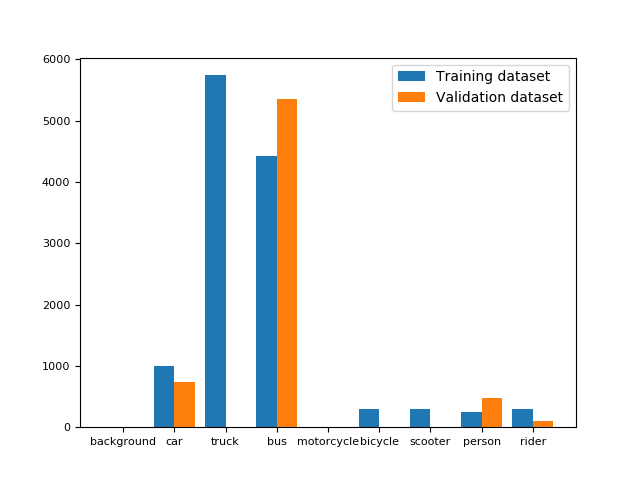
\includegraphics[width=0.49\textwidth]{object_exploration/mean_area.png}}
    \subfigure[]{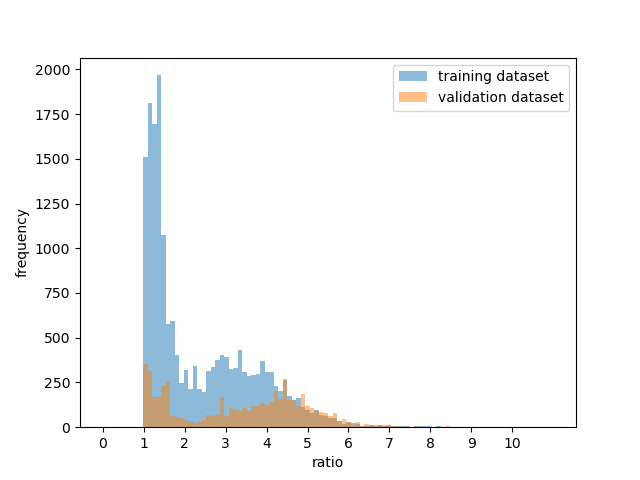
\includegraphics[width=0.49\textwidth]{object_exploration/ratios.png}}
    \caption{Average occurrence of labels (a) in all images (b) in images where the respective label exists.}
    \label{fig:occurrence}
\end{figure}

Extrema:
- image with largest object
- image with highest number of objects
- image with largest number of persons, cars
- minimum number objects - many scooters not annotated

\subsection*{Qualitative analysis}
\begin{itemize}
    \item Are very local features enough or do we need global context? \cite{Karpathy2019}
    \item How much variation is there and what form does it take? 
    \item What variation is spurious and could be preprocessed out? 
    \item Does spatial position matter or do we want to average pool it out? 
    \item How much does detail matter and how far could we afford to downsample the images?
    \item How noisy are the labels? - Labels are correct (for car yes, but is this true for rider, person?) when present, but missing for some objects in a number of images
    \item estimate (mis)predictions and where they might be coming from
\end{itemize}

Points of interest, show sample images, extreme cases

Extreme cases/points of interest:
\begin{itemize}
    \item There are no motorcycles in the dataset
    \item There are no scooters in the validation set
    \item Is the number of riders consistent with the number of vehicles that can transport riders?
    \item Are there motorcycles in the updated dataset?
    \item Many scooters in one place (195, 354) + not annotated!
    \item Large number of rental bikes that were not annotated (images 443, 303)
    \item Just one bicycle annotated, even though several are present in the image: 278
    \item bus not annotated: 0, 42
    \item car (two cars?) not annotated: 99

\end{itemize}

\todo{Show sample images for extreme cases}

\subsection*{Discussion}
\begin{itemize}
    \item Commonalities: The majority of images contain cars (and persons?)
    \item limitations: No motorcycle (due to snow), limited area captured, traffic in recorded area is rarely dense (compared to highways in the US, India, ...)
    \item Missing annotations are bad for performance
    \item Special value of dataset: Captured in one of the most northern parts of the world in winter conditions - evaluate network performance and autonomous driving under the impact of snow
    \item modelling decision derived from exploration:
        \begin{itemize}
            \item Spatial position matters (sensor is moving around landscape is hilly) - random crop for data augmentation meaningful, no average pooling
            \item (delete motorcycle class, as they are no motorcycles in the entire dataset?)
            \item Calibration of $\alpha$ value for focal loss based on label ratios
        \end{itemize}
\end{itemize}

\section*{Task 2: Model Creation}

\subsection*{Task 2.1: Baseline Model}
\begin{itemize}
    \item Technical description of baseline model: short description of changes and reference to code/config files
    \item Quantitative analysis
\end{itemize}

\subsection*{Task 2.2: Data Augmentation}
\begin{itemize}
    \item Report data augmentations used
    \item Quantitative analysis
    \item Compare improvement of data augmentation to Task 2.1
\end{itemize}

\subsection*{Task 2.3}
Focal loss paper: \cite{lin2017focal}

FPN paper: \cite{lin2017feature}

\begin{itemize}
    \item Quantitative analysis after adding each of the four components
    \item References to the code and config file for each component
    \item The four components:
    \begin{enumerate}
        \item Replacing backbone with FPN
        \item Replacing hard-negative mining with Focal loss
        \item Replacing single-layer regression and classification outputs
        \item Initialize bias of last convolutional layer
    \end{enumerate}
\end{itemize}

\subsection*{Task 2.4}
\begin{itemize}
    \item Comprehensive technical description of the modifications introduced to the model in this task: short description of changes and reference to code/config files
    \item Quantitative analysis (?)
\end{itemize}

\subsection*{Task 2.5}
\begin{itemize}
    \item Quantitative analysis on larger dataset
\end{itemize}

\section*{Task 3}

\subsection*{Task 3.1}
Delivered in Task 2 and 4

\subsection*{Task 3.2}
Select three 3 of the most influential modeling decisions throughout the project and present a qualitative analysis. The qualitative analysis should highlight key aspects of your model and should be supported by qualitative
examples.

Example questions that your analysis and discussion can answer are:
\begin{itemize}
    \item What are the strengths of the model?
    \item What are the limitations of the model?
    \item What is the reason that a specific modeling decision improves metric X?
    \item Alternative methods to the modeling decision and why they are better/worse
\end{itemize}

We’ve included a set of scripts to help you to visualize predictions for your qualitative analysis. See the project
readme for more info

\subsection*{Task 3.3}
What are the weaknesses of the approach selected in the project if you were to deliver this to a customer?

\section*{Task 4}

\subsection*{Task 4.1}
Choose two out of the four tasks

\subsection*{Task 4.2}
Choose two out of the four tasks

\subsection*{Task 4.3}
Choose two out of the four tasks

\subsection*{Task 4.4}
Choose two out of the four tasks

\bibliographystyle{alpha}
\bibliography{sample}

\end{document}